\documentclass[9pt]{article}
\usepackage{enumitem}
\usepackage{latexsym}
\usepackage{amsfonts}
\usepackage{float}
\usepackage{fullpage}
\usepackage{graphicx}
\usepackage{geometry}
\usepackage{pdflscape}
\usepackage{booktabs}
\usepackage{listings}
\usepackage{float}
\usepackage{subfigure}
\usepackage{amsmath} % Add the necessary package for the control sequence
\usepackage{setspace} % Add the necessary package for adjusting line spacing
\usepackage{hyperref}
% \usepackage{subcaption}
\geometry{
    left=0.5in,
    right=0.5in,
    top=0.5in,
    bottom=0.5in
}
\newcommand{\N}{\mathcal{N}}
\newcommand{\R}{\mathcal{R}}
\newcommand{\A}{\mathcal{A}}

\newcommand{\handout}[4]{
   \renewcommand{\thepage}{#1-\arabic{page}}
   \pagestyle{empty}
   \noindent
   \begin{center}
   \framebox{
      \vbox{
    \hbox to 6in { {\bf CS657}
         \hfill #2 }
       \vspace{4mm}
       \hbox to 6in { {\Large \hfill #4  \hfill} }
       \vspace{2mm}
       \hbox to 5.78in { {\it #3 \hfill} }
      }
   }
   \end{center}
   \vspace*{4mm}
}

\newcommand{\solheader}[2]{\handout{#1}{\today}{#2}{HW2:Predicting Fake Job Posting}}


%\input{sol_preamble.tex}

% topics: Turing machines, universal TMs, languages, TMs deciding a language, uncomputable languages

\begin{document}
%%%%%%% Edit this next line: parameter 1 is the homework number, the 2nd is your name.
\solheader{1}{Antara Tewary (G01413546),Ankit Kumar (G01436204)}

\begin{enumerate}
    \item \textbf{\underline{Introduction}}\\ 
    This assignment aims to create a system that flags suspicious job postings on Indeed.com, addressing the challenge of fraudulent postings that mislead the efforts of job seekers. We are using Fake Job Prediction Dataset, which contains 18000 job descriptions out of which 800 are fraudulent samples. The goal is to create an automated model which prioritizes which posting to review based on the likelihood of it being fraudulent.
    
    \item \textbf{\underline{Data Preparation}} 
    \begin{itemize}
      \item \textit{Label Encoding and Filtering Invalid Data}: The target column fraudulent was cast to double type to represent legitimate (0) and fake (1) job postings. Any records with invalid values were filtered out.
      \item \textit{Handling Missing Values}:We identified missing values by calculating percentage of null or NaN values across columns and dropped those with more than 1\% null values to reduce noise.
      \item \textit{Text Cleaning}: The job descriptions were cleaned by removing special characters, converting text to lowercase, and removing stop words to ensure uniformity.
      \item \textit{Balancing the Dataset}:
      To address class imbalance, we implemented a custom balancing strategy:
      \begin{itemize}
          \item First, we separated and cached the fraudulent postings (minority class)
          \item Calculated the sampling fraction by dividing the count of fraudulent postings by non-fraudulent postings
          \item Used this fraction to randomly undersample the majority class (legitimate postings) without replacement
          \item Combined the minority class with the sampled majority class using union operation
          \item Randomly shuffled the final balanced dataset to ensure random distribution
      \end{itemize}
      This approach ensured a perfectly balanced dataset while maintaining all fraudulent cases, enabling unbiased model training. The caching of the minority class and random shuffling helped optimize performance and prevent any ordering bias in the final dataset.
    \end{itemize}
    Here are some statistics of the dataset after cleaning:
    \begin{figure}[H]
      \centering
      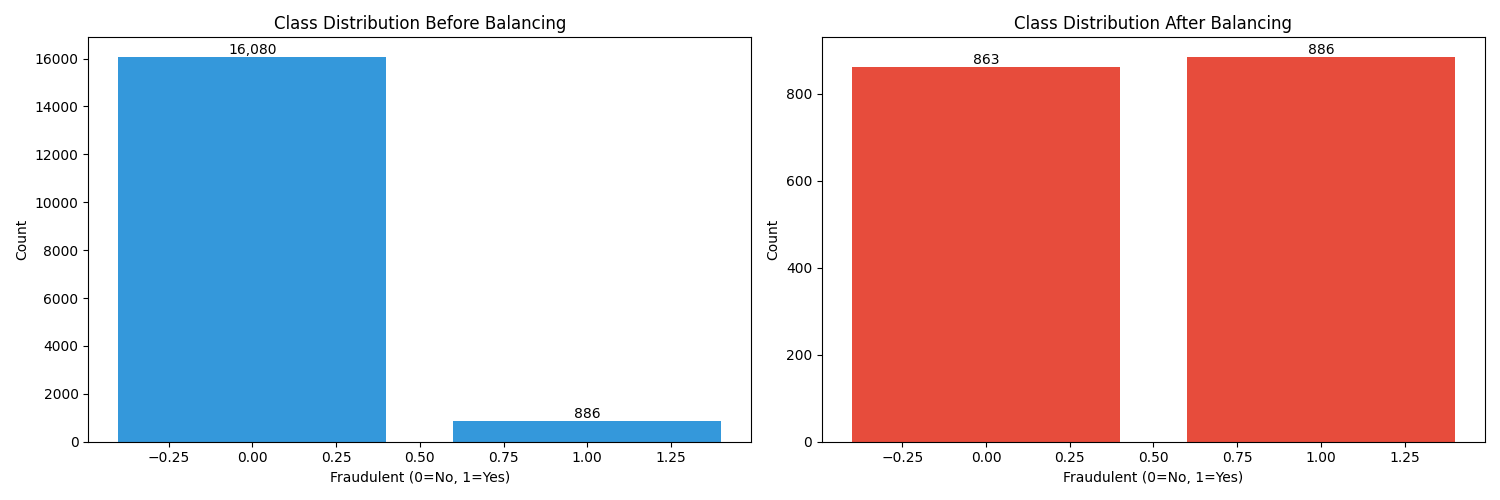
\includegraphics[width=0.8\textwidth]{class_distribution.png}
      \caption{Class distribution before and after balancing}
      \label{fig:class_distribution}
    \end{figure}
    \begin{figure}[H]
      \centering
      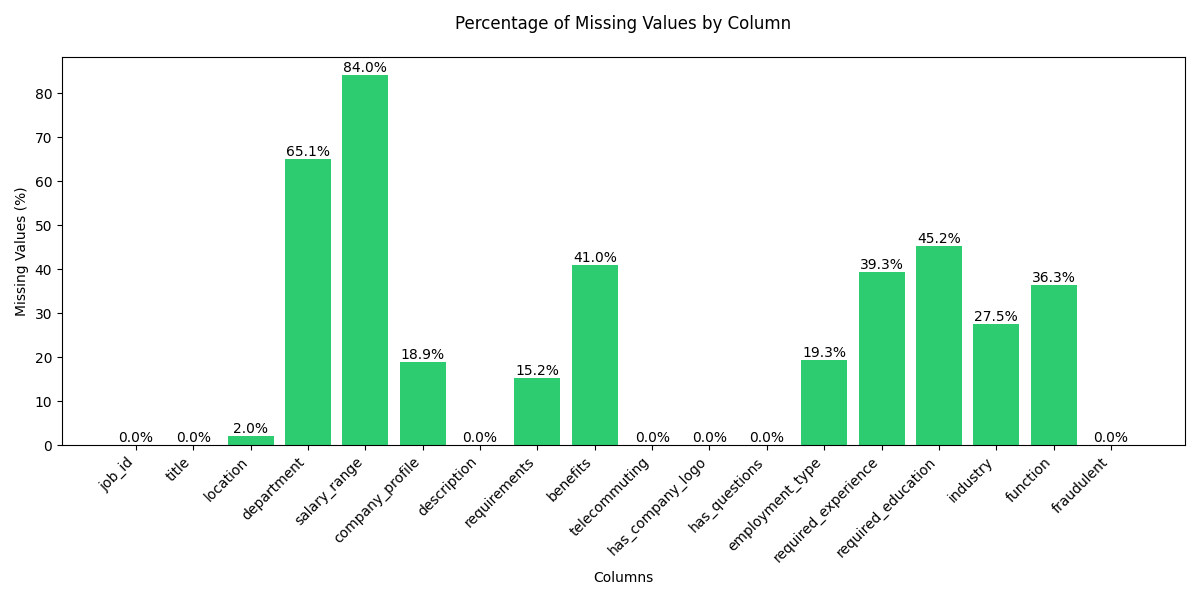
\includegraphics[width=0.8\textwidth]{missing_values.png}
      \caption{\% of missing values for each column}
      \label{fig:class_distribution}
    \end{figure}
  \item \textbf{\underline{Feature Engineering}}\\
  The data contains text features that need to be transformed into numerical representations for model training. We implemented a custom pipeline for processing the job posting text data:
  \begin{itemize}
      \item \textbf{Separate Text Processing}: We processed two key text fields independently,recognizing their different contextual importance.\\
      \textit{Description Processing:}
      \begin{itemize}
          \item Tokenization splits descriptions into individual words, enabling word-level analysis
          \item Stopword removal eliminates common words (e.g., "the", "and"), reducing noise
          \item Count vectorization with a 5000-term vocabulary captures the rich detail in descriptions
          \item Minimum document frequency of 2.0 eliminates rare terms that might represent noise
          \\ 
          \textit{Impact:} This approach preserved the detailed information in job descriptions while reducing dimensionality from unlimited text to a focused 5000-dimension vector.
      \end{itemize}
      \textit{Title Processing:}
      \begin{itemize}
          \item Applied same tokenization and stopword removal
          \item Used a compact 15-term vocabulary using count vectorizer, focusing on key job title terms
          \item Maintained minimum document frequency of 2.0 for consistency
          \\ 
          \textit{Impact:} This concentrated representation captures essential job title information without overwhelming the more detailed description features.
      \end{itemize}
      \item \textbf{Feature Combination and Scaling}
      \begin{itemize}
          \item VectorAssembler combined title (15 dimensions) and description (5000 dimensions) vectors
          \item StandardScaler normalized feature magnitudes while preserving zero elements
          \item Disabled mean centering to maintain vector sparsity
          \\
          \textit{Impact:} This approach:
          \begin{itemize}
              \item Maintains the relative importance of titles vs descriptions
              \item Ensures all features contribute proportionally to model decisions
              \item Preserves memory efficiency through sparse vector representation
          \end{itemize}
      \end{itemize}
  \end{itemize}

  Some statistics after text transformation are shown below:
  \begin{figure}[H]
      \centering
      \subfigure[Text length comparison before and after stopword removal]{
          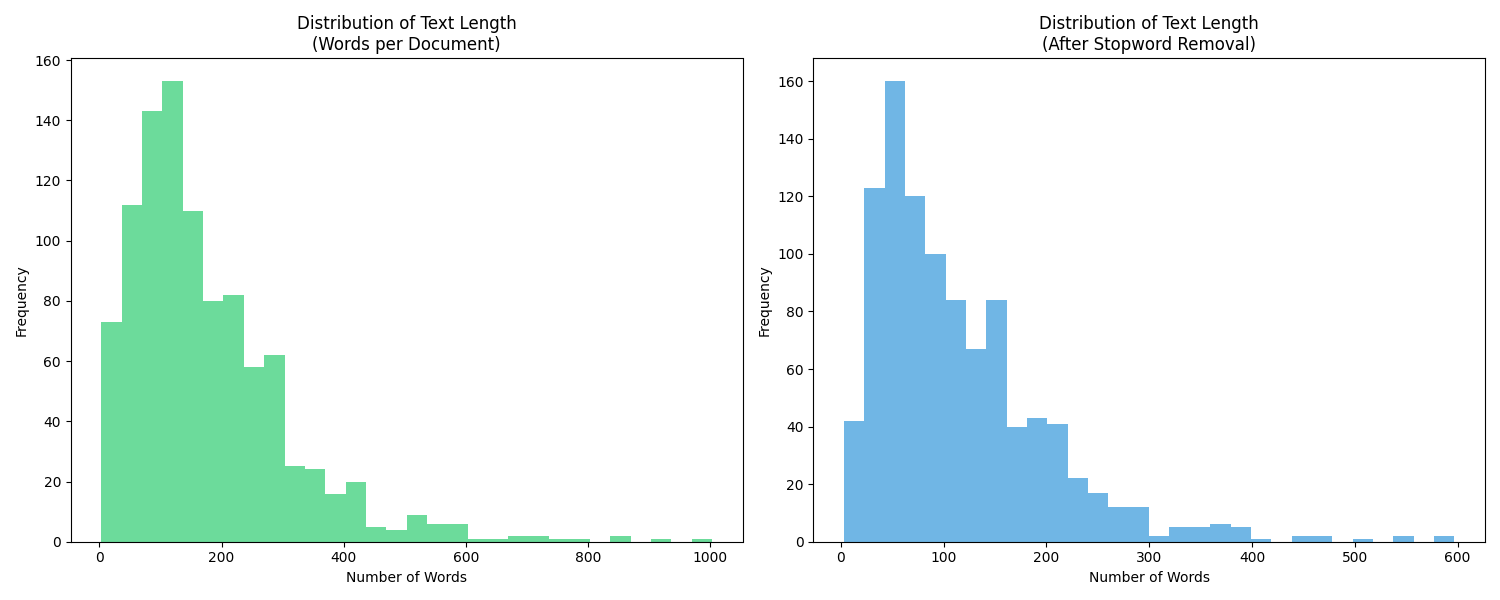
\includegraphics[width=0.7\textwidth]{1_text_length_comparison.png}
          \label{fig:top_words}
      }
      \hspace{0.02\textwidth}
      \subfigure[Top words before and after stopword removal]{
          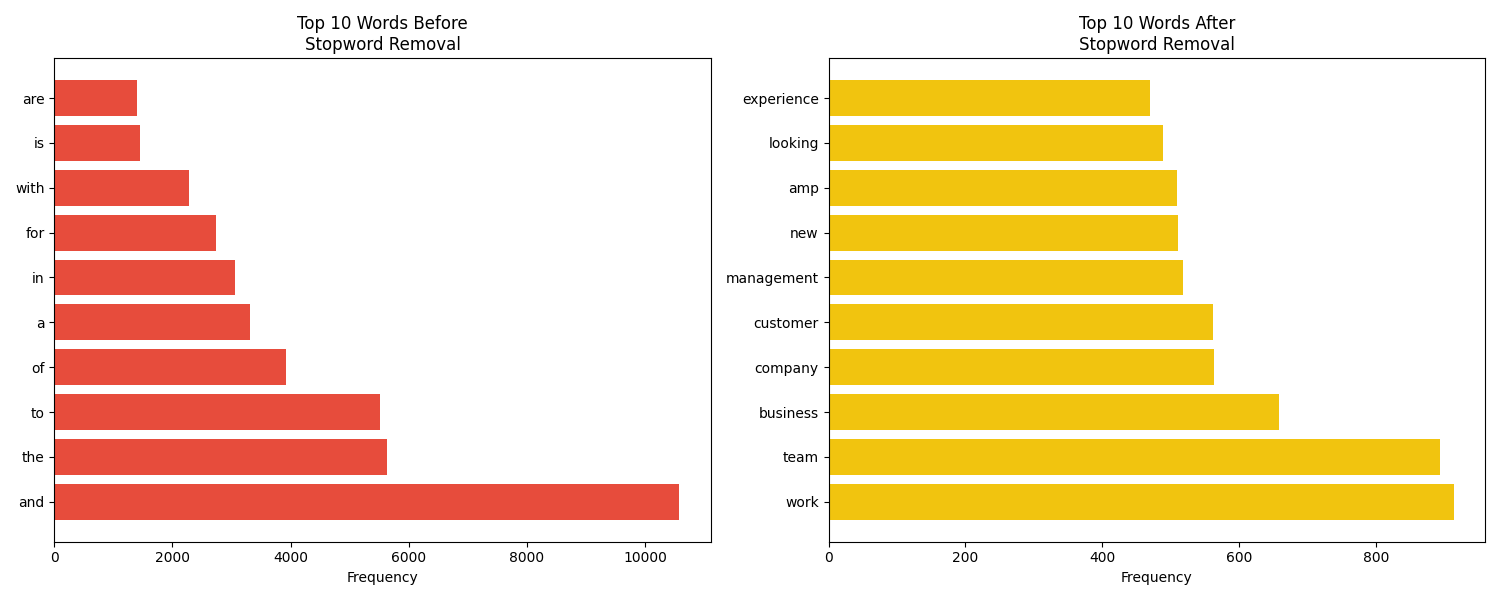
\includegraphics[width=0.7\textwidth]{2_top_words_comparison.png}
          \label{fig:tfidf_distribution}
      }
      \caption{Text Transformation Statistics}
      \label{fig:feature_engineering_statistics}
  \end{figure}
  \item \textbf{\underline{Model Training and Tuning}}\\
  We split the dataset was split into training (70\%) and test (30\%) sets using PySpark's randomSplit function with a seed value of 42 for reproducibility. The dataFrames were cached to optimize performance during model training.
  \begin{itemize}
    \item \textit{Logistic Regression} 
    \begin{itemize}
      \item Trained using a binary classification approach.
      \item Key challenges included handling high-dimensional text features.
      \item Used regularization parameters to prevent overfitting.
      \item Parameters tuned: regularization parameter (0.01-0.3), elastic net mixing (0.0-1.0), and maximum iterations (10-100)
    \end{itemize}
    \item \textit{Linear SVC} 
    \begin{itemize}
      \item Implemented for binary classification of job postings
      \item Focused on finding the optimal hyperplane for classification
      \item Parameters tuned: regularization (0.1-1.0), maximum iterations (10-100), and tolerance (1e-3, 1e-4)
    \end{itemize}
    \item \textit{Random Forest Classifier} 
    \begin{itemize}
      \item Ensemble learning method using multiple decision trees.
      \item Handled high-dimensional feature space effectively
      \item Parameters tuned: number of trees (10-30), maximum depth (5-15), and impurity criterion (gini, entropy)
    \end{itemize}
    \item \textit{Multilayer Perceptron Classifier} 
    \begin{itemize}
      \item Neural network with architecture [num\_features, 20, 2]
      \item Designed for complex pattern recognition in text data
      Parameters tuned: maximum iterations (50, 100), block size (64, 128), and tolerance (1e-4, 1e-5)
    \end{itemize}
    \item \textit{Hyperparameter Tuning} 
    \begin{itemize}
      \item Implemented 10-fold cross-validation for all models
      \item Used ParamGridBuilder for systematic parameter search
      \item Selected hyperparameters focused on:\\
      - Controlling model complexity (regularization parameters)\\
      - Optimization settings (iterations, tolerance)\\
      - Model-specific parameters (trees, depth for Random Forest)
      \item Evaluation metrics: F1 score used as primary metric for cross-validation
      \item Each model was evaluated on both training and test sets to ensure generalization
    \end{itemize}
  \end{itemize}
  \item \textbf{\underline{Model Training and Cross-validation}}\\
  We implemented a comprehensive evaluation of four machine learning models using 10-fold cross-validation on the training set (70\% of data) and final testing on the held-out test set (30\% of data). Each model was tuned using grid search for optimal hyperparameters.

  \begin{itemize}
    \item \textit{Model Performance Summary}:
      \begin{figure}[h]
        \centering
          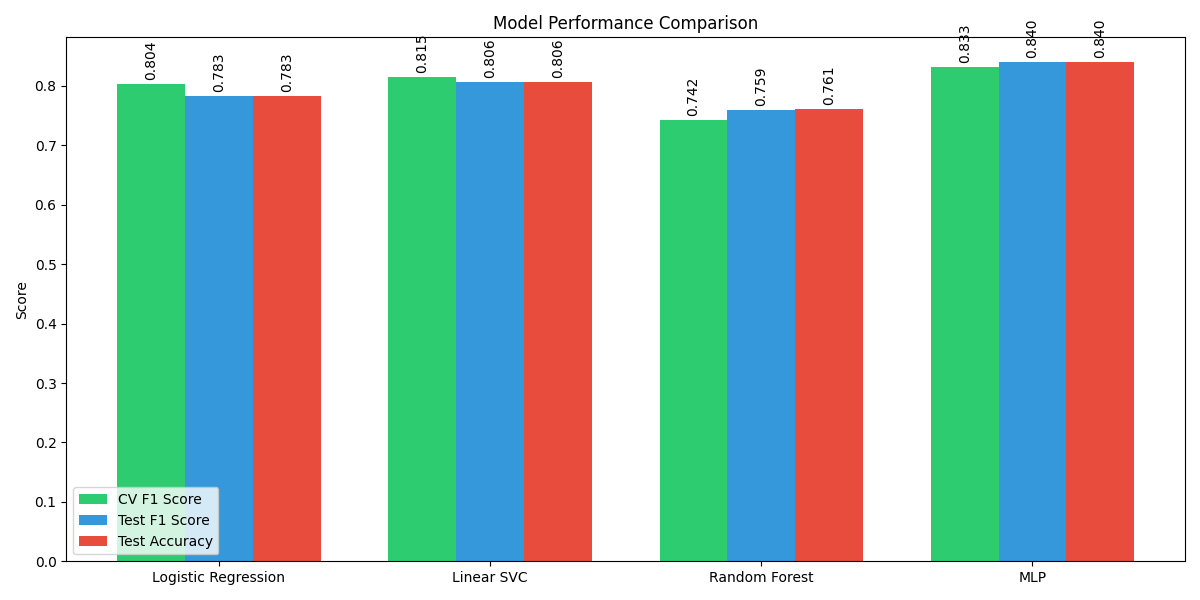
\includegraphics[width=0.8\textwidth]{model_comparison.png}
          \caption{Performance Comparison of Different Models}
          \label{fig:model_comparison}
      \end{figure} 
      \begin{table}[h]
        \centering
        \begin{tabular}{|l|c|c|c|l|}
        \hline
        \textbf{Model} & \textbf{CV F1} & \textbf{Test F1} & \textbf{Accuracy} & \textbf{Best Parameters} \\
        \hline
        Logistic Regression & 0.804 & 0.783 & 0.783 & regParam=0.0, elasticNet=0.0, maxIter=100 \\
        Linear SVC & 0.815 & 0.806 & 0.806 & regParam=0.0, maxIter=100, tol=1e-6 \\
        Random Forest & 0.742 & 0.760 & 0.761 & numTrees=20, maxDepth=5, impurity=gini \\
        MLP Classifier & \textbf{0.833} & \textbf{0.840} & \textbf{0.840} & maxIter=100, blockSize=128, tol=1e-6 \\
        \hline
        \end{tabular}
        \caption{Model Performance and Optimal Parameters}
        \label{tab:model_performance}
        \end{table}     
  \end{itemize}
  \item \textbf{\underline{Conclusion}}
    \begin{itemize}
      \item \textbf{Best Performing Model}: The Multilayer Perceptron Classifier achieved the highest performance with test F1 score and accuracy of 0.840.
      
      \item \textbf{Model Comparison}:
      \begin{itemize}
          \item MLP and Linear SVC showed superior performance ($F1 > 0.80$)
          \item Logistic Regression performed moderately well (F1 $\approx$ 0.78)
          \item Random Forest showed slightly lower performance (F1 $\approx$ 0.76)
      \end{itemize}
      \item \textbf{Consistency}: All models showed good consistency between cross-validation and test performance, indicating robust generalization.
      \item \textbf{Key Insights}
      \begin{itemize}
        \item Neural network-based approach (MLP) demonstrated superior capability in capturing complex patterns in job posting text
        \item Tree-based ensemble method (Random Forest) showed robust performance with simpler implementation
        \item Linear models (SVC and Logistic Regression) performed adequately but were limited in capturing complex text patterns
        \item All models achieved relatively consistent accuracy and F1 score, indicating balanced prediction capabilities
      \end{itemize}
    \end{itemize} 
\end{enumerate}

\end{document}
